\documentclass[mstat,12pt]{unswthesis}

\usepackage{color}
\usepackage{fancyvrb}
\newcommand{\VerbBar}{|}
\newcommand{\VERB}{\Verb[commandchars=\\\{\}]}
\DefineVerbatimEnvironment{Highlighting}{Verbatim}{commandchars=\\\{\}}
% Add ',fontsize=\small' for more characters per line
\usepackage{framed}
\definecolor{shadecolor}{RGB}{248,248,248}
\newenvironment{Shaded}{\begin{snugshade}}{\end{snugshade}}
\newcommand{\AlertTok}[1]{\textcolor[rgb]{0.94,0.16,0.16}{#1}}
\newcommand{\AnnotationTok}[1]{\textcolor[rgb]{0.56,0.35,0.01}{\textbf{\textit{#1}}}}
\newcommand{\AttributeTok}[1]{\textcolor[rgb]{0.13,0.29,0.53}{#1}}
\newcommand{\BaseNTok}[1]{\textcolor[rgb]{0.00,0.00,0.81}{#1}}
\newcommand{\BuiltInTok}[1]{#1}
\newcommand{\CharTok}[1]{\textcolor[rgb]{0.31,0.60,0.02}{#1}}
\newcommand{\CommentTok}[1]{\textcolor[rgb]{0.56,0.35,0.01}{\textit{#1}}}
\newcommand{\CommentVarTok}[1]{\textcolor[rgb]{0.56,0.35,0.01}{\textbf{\textit{#1}}}}
\newcommand{\ConstantTok}[1]{\textcolor[rgb]{0.56,0.35,0.01}{#1}}
\newcommand{\ControlFlowTok}[1]{\textcolor[rgb]{0.13,0.29,0.53}{\textbf{#1}}}
\newcommand{\DataTypeTok}[1]{\textcolor[rgb]{0.13,0.29,0.53}{#1}}
\newcommand{\DecValTok}[1]{\textcolor[rgb]{0.00,0.00,0.81}{#1}}
\newcommand{\DocumentationTok}[1]{\textcolor[rgb]{0.56,0.35,0.01}{\textbf{\textit{#1}}}}
\newcommand{\ErrorTok}[1]{\textcolor[rgb]{0.64,0.00,0.00}{\textbf{#1}}}
\newcommand{\ExtensionTok}[1]{#1}
\newcommand{\FloatTok}[1]{\textcolor[rgb]{0.00,0.00,0.81}{#1}}
\newcommand{\FunctionTok}[1]{\textcolor[rgb]{0.13,0.29,0.53}{\textbf{#1}}}
\newcommand{\ImportTok}[1]{#1}
\newcommand{\InformationTok}[1]{\textcolor[rgb]{0.56,0.35,0.01}{\textbf{\textit{#1}}}}
\newcommand{\KeywordTok}[1]{\textcolor[rgb]{0.13,0.29,0.53}{\textbf{#1}}}
\newcommand{\NormalTok}[1]{#1}
\newcommand{\OperatorTok}[1]{\textcolor[rgb]{0.81,0.36,0.00}{\textbf{#1}}}
\newcommand{\OtherTok}[1]{\textcolor[rgb]{0.56,0.35,0.01}{#1}}
\newcommand{\PreprocessorTok}[1]{\textcolor[rgb]{0.56,0.35,0.01}{\textit{#1}}}
\newcommand{\RegionMarkerTok}[1]{#1}
\newcommand{\SpecialCharTok}[1]{\textcolor[rgb]{0.81,0.36,0.00}{\textbf{#1}}}
\newcommand{\SpecialStringTok}[1]{\textcolor[rgb]{0.31,0.60,0.02}{#1}}
\newcommand{\StringTok}[1]{\textcolor[rgb]{0.31,0.60,0.02}{#1}}
\newcommand{\VariableTok}[1]{\textcolor[rgb]{0.00,0.00,0.00}{#1}}
\newcommand{\VerbatimStringTok}[1]{\textcolor[rgb]{0.31,0.60,0.02}{#1}}
\newcommand{\WarningTok}[1]{\textcolor[rgb]{0.56,0.35,0.01}{\textbf{\textit{#1}}}}


%%%%%%%%%%%%%%%%%%%%%%%%%%%%%%%%%%%%%%%%%%%%%%%%%%%%%%%%%%%%%%%%%%
% 
% OK...Now we get to some actual input.  The first part sets up
% the title etc that will appear on the front page
%
%%%%%%%%%%%%%%%%%%%%%%%%%%%%%%%%%%%%%%%%%%%%%%%%%%%%%%%%%%%%%%%%%

\title{Capstone Project by Team 3\\[0.5cm]A Data Science Approach to
Forecast Short-term Electricity Demand in NSW}

\authornameonly{Karim Adham (z5468227)\\
\strut \\
Rishantha Rajakaruna (z5441528)\\
\strut \\
Rushmila Islam (z5456038) }

\author{\Authornameonly}

\copyrightfalse
\figurespagefalse
\tablespagefalse

%%%%%%%%%%%%%%%%%%%%%%%%%%%%%%%%%%%%%%%%%%%%%%%%%%%%%%%%%%%%%%%%%
%
%  And now the document begins
%  The \beforepreface and \afterpreface commands puts the
%  contents page etc in
%
%%%%%%%%%%%%%%%%%%%%%%%%%%%%%%%%%%%%%%%%%%%%%%%%%%%%%%%%%%%%%%%%%%


\input{header.tex}

\usepackage{booktabs}
\usepackage[table,xcdraw]{xcolor}
\usepackage{colortbl}


\begin{document}

\beforepreface

%\afterpage{\blankpage}

% plagiarism

\prefacesection{Plagiarism statement}

\vskip 2pc \noindent I declare that this thesis is my
own work, except where acknowledged, and has not been submitted for
academic credit elsewhere. 

\vskip 2pc  \noindent I acknowledge that the assessor of this
thesis may, for the purpose of assessing it:
\begin{itemize}
\item Reproduce it and provide a copy to another member of the University; and/or,
\item Communicate a copy of it to a plagiarism checking service (which may then retain a copy of it on its database for the purpose of future plagiarism checking).
\end{itemize}

\vskip 2pc \noindent I certify that I have read and understood the University Rules in
respect of Student Academic Misconduct, and am aware of any potential plagiarism penalties which may 
apply.\vspace{24pt}

\vskip 2pc \noindent By signing 
this declaration I am
agreeing to the statements and conditions above.
\vskip 2pc \noindent
Signed: \rule{7cm}{0.25pt} \hfill Date: \rule{4cm}{0.25pt} \\[1cm]
\vskip 1pc

%\afterpage{\blankpage}

% Acknowledgements are optional


\prefacesection{Acknowledgements}

{\bigskip}TBW\ldots{}\\[1cm] 

{\bigskip\bigskip\bigskip\noindent} 02/10/2024.

%\afterpage{\blankpage}

% Abstract

\prefacesection{Abstract}

TBW \ldots{}

%\afterpage{\blankpage}


\afterpreface





%%%%%%%%%%%%%%%%%%%%%%%%%%%%%%%%%%%%%%%%%%%%%%%%%%%%%%%%%%%%%%%%%%
%
% Now we can start on the first chapter
% Within chapters we have sections, subsections and so forth
%
%%%%%%%%%%%%%%%%%%%%%%%%%%%%%%%%%%%%%%%%%%%%%%%%%%%%%%%%%%%%%%%%%%



%%%%%%%%%%%%%%%%%%%%%%%%%%%%%%%%%%%%%

%\afterpage{\blankpage}


\chapter{Introduction}\label{introduction}

Accurate Electricity demand forecasting is a fundamental component of
decision making for governments, regulatory bodies and businesses. To
forecast electricity demand we need to understand the drivers of demand
fluctuation and corresponding relationships. Weather changes, long-term
climate change and macroeconomic influences such as, population growth,
economic growth are key factors that influence demand \cite{a2024_nem}.
Additionally, generation of electricity through renewable sources such
as Solar and Wind which doubled over the last decade has added more
complexity to forecasting due to its dependency on weather
\cite{energygovau_2024_renewables}.

The demand forecasting varies from short term to medium and long term.
The parameters that influence each period type varies. Short term
forecasting focus on small time intervals. i.e.~few minutes upto few
days. It can be heavily influenced by daily weather, time of the day and
holidays. In case of medium to long term forecast, the timeframe could
vary from few months to few years into the future and determined by long
term factors such as climate change, population growth, government
policy to name a few.

This research paper focus on short term forecasting. Therefore,
primarily use half hourly temperature, historical half hourly actual
demand, calendar information (holidays, weekends) and time of the day as
key data sources. We analyse in detail the relationship between demand
and the aforementioned features and use two models, \textbf{XGBoost} and
\textbf{Prophet by Facebook} to forecast daily demand.

By using multiple matrices, we compare the performance of each model.
Additionally, we also compare the results of the two models against the
short-term demand forecast published by Australian Energy Market
Operator.

We hope the findings will assist market participants to make informed
decisions with regards to short term electricity demand forecasting and
contribute to a more sustainable and efficient energy landscape.

\bigskip

\chapter{Literature Review}\label{literature-review}

\section{Background}\label{background}

Electricity demand forecasting is crucial for ensuring an efficient,
reliable and cost-effective power operation systems. Accurate forecasts
enable grid operators to balance supply and demand in real-time,
preventing costly overproduction or dangerous shortages that could lead
to blackouts. It also helps to optimize the scheduling of power
generation for different sectors, reducing operational costs and
enhancing system reliability. As renewable energy sources like solar and
wind become more integrated, forecasting plays a vital role in managing
fluctuations in supply. Additionally, in deregulated markets, precise
demand predictions allow energy providers to make informed trading
decisions, ultimately benefiting both suppliers and consumers with more
stable and affordable electricity.

According to \cite{nsw_epa_2021_energy_consumption} electricity demand
from the NSW grid is projected to experience a slight decline over the
next five years before rising more. As stated in the article the main
reason for the decline in energy consumption is the lower consumption by
the NSW industrial sector, particularly the manufacturing industry,
population growth being by improvements in the energy efficiency of
appliances and machinery. In addition, the increasing adoption of
rooftop solar panels and battery storage systems is anticipated to
further lower residential demand on the electricity grid. Beyond the
five-year mark, consumption is forecasted to increase as electric
vehicle charging and broader electrification begin to significantly
impact electricity demand. In the Figure \ref{renewable} we can
visualize the rapid growth of electricity generation using renewable
sources.

\begin{figure}[H]
\centering
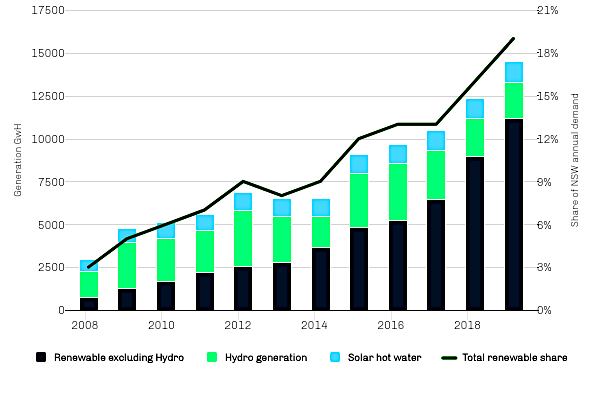
\includegraphics[width=0.95\textwidth,height=10cm]{renewable_fuel_sources_chart.png}
\caption{Renewable fuel sources [Source:
Derived from Department of the Environment and Energy, Australian Energy Statistics, Table O, June 2021]}\label{renewable}
\end{figure}

NSW is predominantly self-sufficient in relation to electricity supply
according to \linebreak \cite{nsw_epa_2021_energy_consumption}, relying
on state generation to meet local demand with additional electricity is
imported from other states through the National Electricity Market (NEM)
to optimize costs for the consumers. In 2019--20, renewable energy
sources accounted for approximately 19\% of the state's total
electricity generation, a significant increase from past years. Accurate
demand prediction is critical for ensuring optimal resource allocation
and cost management, particularly as the state integrates more renewable
energy into its supply mix.

\section{Factors Affecting Load
Forecasting}\label{factors-affecting-load-forecasting}

Load forecasting is usually concerned with the prediction of hourly,
daily, weekly, and annual values of the system demand and peak demand.
Such forecasts are sometimes categorized as short-term, medium-term and
long-term forecasts, depending on the time horizon. In terms of
forecasting outputs, load forecasts can also be categorized as point
forecasts (i.e., forecasts of the mean or median of the future demand
distribution), and density forecasts (i.e., estimates of the full
probability distributions of the possible future demand values).

As stated in \cite{nsw_epa_2021_energy_consumption} the driving factors
of electricity consumption and demand forecasts can be split into two
different types: ---1) structural like population growth, economic
condition, electricity price, energy efficiency etc; and 2)
non-structural or random like weather condition e.g., air temperature,
extreme heat or cold, bushfire, flood, etc., building type e.g.,
multi-storey or free-standing house, and adoption of electric vehicles
and contributions of renewable energy in the power grid, etc. There are
many factors that drive consumers to make similar choices regarding
electricity consumption at the same time like work and school schedules.
The demand is different during weekdays, public holidays, weekends, due
to weather the use of heating and cooling appliances, and many other
societal factors, such as whether the beach is pleasant, or the
occurrence of retail promotions.

Temperature is a crucial factor, as it directly influences electricity
consumption patterns. Extreme temperatures, whether very hot or cold,
can lead to higher demand for heating or cooling, respectively.
Forecasts often need to account for temperature variations to predict
demand more accurately, especially during seasonal extremes or unusual
weather patterns.

\begin{figure}[H]
\centering
\includegraphics[width=0.95\textwidth, height=10cm]{extreme_temp__au.png}
\caption{The frequency of extreme heat events in Australia from 2010 to 2020}\label{extreme}
\end{figure}

Figure \ref{extreme} shows the overall temperature rise in Australia and
forecast shows that it will continue to rise. The climate of NSW is
changing, with 6 of the 10 warmest years on record occurring in the past
10 years \cite{nswAdaptNSW}. The warmest year on record in NSW was 2019,
with on average temperature of 1.2°C above the 1990--2009 average.
Across NSW, average temperatures will continue to increase throughout
this century and by 2090, average temperature is projected to rise by
around 1.3°C under a low emissions scenario and around 4.0°C under a
high emissions scenario. So temperature is key factor while determining
the electricity demand as fluctuations in heating and cooling usage
drive consumption patterns. Colder nights lead to increased heating,
while hot days cause a spike in cooling system usage. These variations
directly impact electricity demand, making accurate short-term forecast
is very crucial for grid operators to manage supply and demand
effectively.

Holidays and weekdays are also important key factors in load
forecasting. On holidays, electricity consumption patterns can differ
significantly from regular weekdays due to changes in work routines and
social activities. For instance, public holidays might see a decrease in
commercial and industrial electricity use, while residential usage could
increase due to family gatherings and home activities.

Incorporating temperature data and considering holiday effects are
essential for creating more accurate and reliable electricity demand
forecasts, which in turn support better decision-making for power system
management and operational planning.

\section{Electricity Demand Forecast
Methodologies}\label{electricity-demand-forecast-methodologies}

Electricity demand or load forecasting is a well-known problem that
involves predicting future load based on historical information.
Econometric models and time series models are the most commonly used
classical load forecasting techniques. These approaches rely on past
observations to project future demand. As mentioned in \cite{9812604}
econometric approach combines statistical techniques with economic
theory to estimate the relationship between influencing factors and
energy consumption, enabling a deeper understanding of how various
factors - such as economic conditions and weather - impact electricity
demand across industrial, residential, and commercial sectors. The
econometric approach uses historical data to provide comprehensive
insights into future trends and the reasons behind them. However,
despite its advantages, it may not fully capture the interdependence
between quantity and prices, limiting its forecasting accuracy in
certain cases. On the other hand, time series models focus on analyzing
historical load data to identify patterns and predict future values
based solely on past trends. These models offer structural simplicity,
as they rely entirely on previous observations to forecast future
demand. While effective for forecasting, they do not explain cause and
effect relationships between variables, thus limiting their ability to
account for changes in underlying factors.

Researchers used both statistical and probabilistic methods to achieve
high accuracy with low errors to find the best model. They also
considered this problem as both deterministic and stochastic to include
the influence of the external factors that sways the models behavior at
different time horizons. As mentioned in \cite{9812604} load forecasting
on the basis of time horizon, can be classified into four forecasting
groups -- VSLTF (very short-term load forecasting), STLF (short-term
load forecasting), MTLF (medium-term load forecasting), and LTLF
(long-term load forecasting).

\begin{itemize}
\item
  VSTLF: This is used to forecat from minutes to hour (0-3h). It can
  deal with random variations in renewable energy production and demand.
  It is used for the purpose of real-time operation and control of the
  grid.
\item
  STLF: This method is used for forecasting ahead of few minutes to few
  days. It has a key role in different grid operations involving
  reliability analysis and dispatch analysis. Further, it helps to avoid
  over estimation and under estimation of the energy demand and thus
  contribute substantially in the reliability of grid.
\item
  MTLF: In this method time scale expands from few days to months ahead
  during a year. It helps maintenance, adequacy assessment and fuel
  supply in smart grid systems. Further, it plays an important role to
  evaluate the financial attributes of energy system by contributing to
  risk management.
\item
  LTLF: This forecasting method involves time scale ranging from months
  to even years. LTLF is very important for every production and load
  growth planning operations for long duration of time. The big
  advantage of LTLF is that it can remove the effects of random
  fluctuations occur in short term and make the prediction of long term
  trends.
\end{itemize}

As mentioned in \cite{9812604}, there are methods for VSTLF including
genetic algorithm, autoregressive moving average models and artificial
neural network. STLF is utilized for time hardly from minutes to hours.
STLF is the important source of information for daily operations and it
is important for system operations. Researchers are taking more interest
to design predictive models because STLF can be used to approximate the
long time load. It is essential to have accurate predict knowledge of
affecting factors to improve short term model. For duration of days to
months, usually MTLF is used for load forecasting. It becomes popular in
peak summer or winter. For load duration from few weeks to many years,
LTLF is considered. The factors including weather data, characteristics
of install devices at areas of interest, history of load and numbers of
customers are accounted in it. The factors of economic are taken into
account for long period methods of load forecasting. The Table
\ref{forecasting_methods} \cite{9812604} below shows the different load
forecasting methods and their characteristics.

\begin{table}[h]
\caption{Forecasting methods}
\centering
\resizebox{\textwidth}{!}{
\begin{tabular}{c|c|c|c|c|c}
\hline \hline
 &  &  & Factors &  &  \\ 

Methods &  Time  Duration &  Temperature & Economics & Use of land & Usases \\ \hline
VSTLF & Few minutes & Not compulsory & Not compulsory & Not compulsory & To generate forecasting. \\ \hline
STLF & Few hours & Compulsory & Not compulsory & Not compulsory & Distribution schedule. \\ \hline
MTLF & Days to months & Simulated & Compulsory & Not compulsory & Maintenance schedule. \\ \hline
LTLF & More than year & Simulated & Simulated & Compulsory & Allocation of spinning reserve. \\ \hline
\end{tabular}
}
\label{forecasting_methods}
\end{table}

Based on the required time horizons we can further classify the problem
into three broad solution domains - heuristic, statistical or
econometric, and probabilistic models. Time series datasets have the
unique property of dependence on what happened in the past. Therefore,
we cannot randomly shuffle the order of the data without affecting the
trends. With such dependency simple regression technique for forecasting
can randomly show statistical significance even if there is no true
correlation, and thus suitable for real-world usage. In the following
sections, we will discuss the popular forecasting models used in the
electricity demand forecasting domain.

\section{Forecasting Models}\label{forecasting-models}

Various techniques have been developed for electricity demand
forecasting during the past few years. Electricity load forecasting
models can be classified into parametric, semi-parametric, and
non-parametric models based on the assumptions they make about the
underlying data distribution and the flexibility in capturing
relationships between variables. Parametric models rely on a fixed,
predefined functional form with a finite number of parameters. For
example linear regression, ARIMA, and exponential smoothing models,
assume a specific relationship between predictors (e.g., temperature,
time) and load. These models are easy to interpret but less flexible
when dealing with complex or non-linear patterns in the data. As
discussed in \cite{Fan2012}, statistical models are widely adopted for
the load forecasting problem, which include linear regression models,
stochastic process models, exponential smoothing and ARIMA models.

Semi-parametric models, such as Generalized Additive Models (GAMs),
combine both parametric and non-parametric components. They allow for
linear relationships between some variables while using smoothing
functions to capture non-linear effects, offering a balance between
interpretability and flexibility. A more recent and very popular GAM for
regression technique is Prophet \cite{taylor2017facebook}. It is
designed to optimally handle business forecasting tasks featuring time
series captures at the hourly, daily, or weekly level with ideally at
least a full year of historical data.

Finally, non-parametric models like Random Forests, Support Vector
Regression (SVR), k-Nearest Neighbors, and Artificial Neural Networks
(ANN) do not assume any specific form for the relationship between
inputs and outputs. These models are highly flexible and can model
complex, non-linear interactions but are more computationally intensive
and can be harder to interpret compared to their parametric
counterparts. Each class of models has it's strengths, with the choice
depending on the data complexity and the forecasting objectives.
Recently, machine learning techniques and fuzzy logic approaches have
also been used for load forecasting or classification and achieved
relatively good performances. ANN have been shown to have the ability
not only to learn the load series but also to model an unspecified
nonlinear relationship between load and weather variables.

\begin{table}[h]
  \caption{Forecasting methods}\label{tab:forecasting_methods1}
    \scalebox{0.9}{
    \centering
    \begin{tabular}{|c|p{5cm}|p{6cm}|} % 'p{5cm}' specifies the column width
        \hline
        Forecasting methods & Advantages & Disadvantages\\ 
        \hline
        Statistical methods & 
        Uncomplicated and less computionally expensive. & 
        Less reliablity for large and non-linear dataset.  \\ 
        \hline
        Machine learning & 
        Simple and can deal with large dataset. & 
        Less reliable for large heterogenous data and produce point prediction.\\ 
        \hline
        Deep learning & 
        Efficient for large non-linear dataset. & 
        Creates point prediction, overfitting needs hyper-parameter tuning.\\ 
        \hline
        SVM & 
        Overfitting is handled with regularization. NO local minima and many effective methods to solve problem.& 
        Dependency on kernal and has slow testing process.\\ 
        \hline
        Time series analysis & 
        Quick and accurate execution.& 
        Numerical instability.\\ 
        \hline
    \end{tabular}
    }
    %\caption{Example of Text Wrapping in a LaTeX Table}
\end{table}

Now, let's examine which models are most appropriate for different
forecasting problems based on the time horizon involved. For short-term
forecasting, covering hours to a few days, models that integrate
external factors such as weather conditions, time of day, and social
behaviour become critical. Generalized Additive Models (GAMs) and
Support Vector Machines (SVMs) are often applied for their ability to
account for non-linear relationships between demand and influencing
variables like temperature, day of the week, and holidays. Hybrid
models, which combine machine learning techniques with statistical
methods like exponential smoothing or seasonal ARIMA, are also effective
for this timeframe, as they can capture both the short-term trends and
seasonal patterns inherent in electricity
consumption.\newline \cite{Wang2021} highlights that although these
traditional techniques such as fuzzy linear regression, exponential
smoothing, Automatic Regressive Moving Average (ARMA) have the
advantages of algorithmic simplicity but they are not scalable to handle
large dataset and model complicated relationships. Popular machine
learning model XGBoost is widely regarded as a powerful tool for
short-term load forecasting due to its ability to handle large dataset
and model complex non-linear relationships efficiently. Studies have
demonstrated that XGBoost can outperform traditional neural networks in
terms of both accuracy and computational speed, especially when dealing
with tabular data, such as historical electricity demand {[}???Ref{]}.
\textbf{RNNs} are commonly used for load forecasting when there is a
need to model temporal dependencies over shorter sequences. They are
effective in predicting short-term fluctuations in electricity demand,
especially when there is a clear trend or pattern over recent time
intervals, such as hourly or daily demand variations. However,
traditional RNNs suffer from the vanishing gradient problem, which
limits their ability to retain information over long time sequences.
This makes them less effective for capturing long-term dependencies or
seasonal patterns in electricity consumption. To overcome the
limitations of RNNs, \textbf{LSTM networks} are often preferred for load
forecasting, especially when dealing with longer time horizons or when
it's important to capture both short-term and long-term trends in
electricity demand. LSTM networks are designed with a memory cell that
can store information for extended periods, allowing the model to retain
past information over long time sequences. This makes LSTMs particularly
effective for \textbf{short-term to medium-term forecasting}, where
demand patterns depend on both recent trends (such as hourly or daily
fluctuations) and more distant patterns (such as weekly or seasonal
cycles). One of the main shortcomings of using LSTM in short-term load
forecasting is its tendency to overfit when the model complexity
increases, especially with limited training data. Additionally, LSTM
models often require significant computational resources and long
training times, which can be less efficient for real-time applications
where immediate predictions are crucial {[}???REF{]}. Medium-term
forecasting, which spans weeks to months, focuses on predicting
consumption patterns based on broader trends, such as seasonal
variations, economic cycles, and energy market dynamics. Time-series
models like SARIMA (Seasonal ARIMA) and Exponential Smoothing State
Space (ETS) models are widely used for their ability to capture seasonal
effects and trends. Additionally, machine learning techniques like
Gradient Boosting Machines (GBM) or Random Forests can be leveraged to
include more complex interactions between variables, such as the effect
of emerging technologies like rooftop solar panels. These models are
crucial for tasks such as planning maintenance or scheduling energy
generation resources. For long-term electricity demand forecasting,
\textbf{econometric models} and \textbf{scenario based models} are often
preferred over short-term forecasting methods like neural networks. This
is because long-term forecasting, which spans months to years, requires
capturing structural trends, external factors, and macroeconomic
indicators that influence electricity demand over extended periods.

\section{Challenges to Find the Ideal Electricity Load Forecasting
Method}\label{challenges-to-find-the-ideal-electricity-load-forecasting-method}

In this study we focus on short-term demand forecasting which is an
essential instrument in power system planning, operations, and control.
Many operating decisions are based on load forecasts such as dispatch
scheduling of generating capacity, reliability analysis, and maintenance
planning for the generators. Overestimation of electricity demand will
cause a conservative operation which may lead to overproduction or
excessive energy purchase. For instance, in \cite{AEMO} AEMO uses a
monthly regression model based on five years (60 months) of historical
data and the choice of five years data strikes a balance between
ensuring that the model considers only relatively recent univariate
consumption trends and behaviours while being long enough to capture
seasonality and contain enough multivariate observations to be
statistically meaningful. Univariate models, while simpler, often
struggle to capture complex relationships and seasonal patterns in load
data. Multivariate models, incorporating additional factors like
temperature, humidity, and economic indicators, can improve accuracy but
introduce challenges in data collection, preprocessing, and model
complexity, thus require careful feature engineering. Univariate models
use only historical demand data to make future predictions, while
multivariate models consider other variables such as atmospheric
variations and calendars along with historical demand data in the study
of STLF \cite{asi6060100}, \cite{wang2016review} and
\cite{chen2015electricity} both highlight the limitations of traditional
methods and the growing interest in advanced hybrid techniques.
Therefore, the selection of an ideal forecasting method depends on
factors such as data availability, computational resources, and the
desired level of accuracy, making it a complex and ongoing research
area.

\cite{taylor2009forecasting} developed both univariate and multivariate
models and stated that the univariate models had good prediction
capability. In univariate time series models, the historical electricity
demand data are arranged with correlated past lags to capture the demand
patterns even when the data are limited. \cite{mcculloch2001forecasting}
obtains improved accuracy by including the temperature as a variable,
recognising that weather conditions play a crucial role in forecasting
performance. \cite{Fan2012} proposes a semi-parametric additive models
to estimate the relationships between demand and the driver variables.
Specifically, the inputs for these models are calendar variables, lagged
actual demand observations and historical and forecast temperature
traces for one or more sites in the target power system. The proposed
methodology has been used to forecast the half-hourly electricity demand
for up to seven days ahead for power systems in the Australian National
Electricity Market (NEM). To achieve more efficient and accurate load
forecasting \cite{Suo} establishes a multi-dimensional short-term load
forecasting model based on XGBoost. The decision forest composed of many
decision trees is the final learning model of XGBoost. It tries to
correct the residual of all the previous weak learners by adding new
weak learners. When these learners are combined for final prediction the
accuracy will be higher than that of a single learner. The selection of
appropriate hyper parameters of XGBoost is directly related to the
performance of the model but there is no universal and scientific method
to determine the hyper parameters. In order to reduce the randomness and
blindness, based on the second search of multi-dimensional grids, a
method of hyper parameters optimisation is proposed. Each hyper
parameters combination is attempted in a grid traversal manner in turn.
In short-term demand forecasting, faster computation is essential due to
the need for real-time or near-real-time predictions. Models like
XGBoost are preferred over LSTM because of their speed and ability to
handle large dataset, faster training time and higher interpretability.
However, limitations in computational power can impact the selection of
models and their performance. This is especially critical when dealing
with complex models or large-scale data, where ensuring optimal
performance within available resources becomes a trade-off between
prediction accuracy and computational feasibility.

\section{Performance Metrics and Model
Evaluations}\label{performance-metrics-and-model-evaluations}

To check the correctness of the methods used for the prediction of real
values of load, different criteria are utilized to evaluate the
techniques of load forecasting. The research of many researchers based
on statistical metrics to optimize the precision of their model, newly
developed statistical metrics such as probabilistic load forecasting
metrics. Due to wide adaptation and extraordinary academic values in
industry, literature on probabilistic forecasting is still in developing
phase. The most important static metrics used by researchers are shown
below:

\begin{table}[h]
\centering
\caption{Formula Table}
\begin{tabular}{|c|c|}
\hline
\textbf{Name of criteria} & \textbf{Formula} \\ 
\hline
Mean Absolute Error (MAE) & $\frac{\sum_{i=1}^n|\hat{y_i}-y_i|}{n}$ \\ 
\hline
Root Mean Square Error (RMSE) & $\sqrt{\frac{1}{n}\sum_{i=1}^{n}(\hat(y_i) - y_i)^2}$ \\ 
\hline
Mean Percentage Error (MAE) & $\frac{1}{n}\sum_{i=1}^{n}\frac{(y_i-\hat{y_i})}{y_i}$ \\ 
\hline
\end{tabular}
\end{table}

To report performance the most basic method, \emph{hold-out} validation
and split the data to 80/20 split for training and testing or 60/20/20
for training/validation/testing. The other approach to evaluate the
performance of the model using cross-validation. As discussed in
\cite{rafferty2023forecasting}, the traditional k-fold cross-validation
technique is not suitable for time series data because it shuffles the
data randomly and does not take into account the temporal structure of
the data. Instead, time series cross-validation methods like forward
chaining or rolling-origin cross validation which is similar to k-fold
cross-validation but maintains the temporal order of the data. In this
research study we will explore the hold-out validation, k-fold and
forward chaining cross-validation technique to evaluate the performance
of the models.

\chapter{Material and Methods}\label{material-and-methods}

\section{Software}\label{software}

Primary software used for analysis and model build is Python. We have
used extensive set of python libraries. List of libraries used are,

\begin{itemize}
  \item holidays - Derive public holidays in NSW 
  \item pandas - Data selection and manipulation
  \item numpy - Calculations and data manipulation
  \item statsmodels - Used for statistical tests and statistical data exploration
  \item matplotlib, seaborn - To create plots and visualize statistical analysis
  \item scipy - statistical analysis
  \item sklearn - Model preparation and analysis
  \item xgboost - Used for XGBoost model build
  \item prophet - Used for Facebook Prophet model build
\end{itemize}

Jupyter Notebook and RStudio was used as integrated development
environments. Github repository was used for code management. Teams and
One Drive were used for collaboration and communication.

\section{Description of the Data}\label{description-of-the-data}

\begin{enumerate}
    \item Total Electricity Demand NSW
    \item Air Temperature NSW
    \item NSW Calendar
    \item Total Forecast Demand NSW
\end{enumerate}

\subsection{Total Electricity Demand
NSW}\label{total-electricity-demand-nsw}

Total Electricity Demand in 30 min increments. This data is sourced from
the Market Management System database, which is published by the market
operator from the National Electricity Market (NEM) system and
downloaded from \cite{UNSW_project}.

\begin{table}[h]
\tiny
\begin{tabular}{@{}|l|l|l|l|@{}}
\toprule
\textbf{Row Count} & \textbf{File Size (Approx)} & \textbf{File Format} & \textbf{File Name}   \\ \midrule
196513             & 5.6 MB                      & CSV                  & totaldemand\_nsw.csv \\ \bottomrule
\end{tabular}
\end{table}

\begin{table}[h]
\tiny
\begin{tabular}{@{}|l|l|l|@{}}
\toprule
%\rowcolor[HTML]{EFEFEF} 
\textbf{Attributes} & \textbf{Description}                                                                                             & \textbf{\begin{tabular}[c]{@{}l@{}}Attribute \\ Characteristics\end{tabular}} \\ \midrule
DATETIME            & \begin{tabular}[c]{@{}l@{}}Date and time interval of each observation. \\ Format (dd/mm/yyyy hh:mm)\end{tabular} & Timestamp                                                                     \\ \midrule
TOTALDEMAND         & Total demand in MW                                                                                               & Numeric                                                                       \\ \midrule
REGIONID            & Region Identifier (i.e. NSW1)                                                                                    & \begin{tabular}[c]{@{}l@{}}String.\\ Categorical\end{tabular}                 \\ \bottomrule
\end{tabular}
\end{table}

\subsection{Air Temperature NSW}\label{air-temperature-nsw}

Air temperature in NSW (as measured from the Bankstown Airport weather
station). This data is sourced from the Australian Data Archive for
Meteorology. Note: Unlike the total demand and forecast demand, the time
interval between each observation may not be constant (i.e.~half-hourly
data). As noted in the literature review, temperature is a key driver of
demand. Therefore, this dataset is critically important for the research
question.

\begin{table}[h]
\tiny
\begin{tabular}{@{}|l|l|l|l|@{}}
\toprule
%\rowcolor[HTML]{EFEFEF} 
\textbf{Row Count} & \textbf{File Size (Approx)} & \textbf{File Format} & \textbf{File Name}   \\ \midrule
220326             & 6.7 MB                      & CSV                  & temperature\_nsw.csv \\ \bottomrule
\end{tabular}
\end{table}

\begin{table}[h]
\tiny
\begin{tabular}{@{}|l|l|l|@{}}
\toprule
%\rowcolor[HTML]{EFEFEF} 
\textbf{Attributes} & \textbf{Description}                                                                                             & \textbf{\begin{tabular}[c]{@{}l@{}}Attribute \\ Characteristics\end{tabular}} \\ \midrule
DATETIME            & \begin{tabular}[c]{@{}l@{}}Date and time interval of each observation. \\ Format (dd/mm/yyyy hh:mm)\end{tabular} & Timestamp                                                                     \\ \midrule
TEMPERATURE         & Air temperature (°C)                                                                                             & Numeric                                                                       \\ \midrule
LOCATION            & 